\begin{abstract}
This work aims to address the multi-view perspective RGB generation from text prompts given Bird-Eye-View(BEV) semantics. Unlike prior methods that neglect layout consistency, lack the ability to handle detailed text prompts, or are incapable of generalizing to unseen view points, MVPbev simultaneously generates cross-view consistent images of different perspective views with a two-stage design, allowing object-level control and novel view generation at test-time. Specifically, MVPbev firstly projects given BEV semantics to perspective view with camera parameters, empowering the model to generalize to unseen view points. Then we introduce a multi-view attention module where special initialization and de-noising processes are introduced to explicitly enforce local consistency among overlapping views w.r.t. cross-view homography. Last but not the least, MVPbev further allows test-time instance-level controllability by refining a pre-trained text-to-image diffusion model. Our extensive experiments on NuScenes demonstrate that our method is capable of generating high-resolution photorealistic images from text descriptions with thousands of training samples, surpassing the state-of-the-art methods under various evaluation metrics. We further demonstrate the advances of our method in terms of generalizability and controllability with the help of novel evaluation metrics and comprehensive human analysis.%\footnote{Our code, data and model can be found in \url{https://github.com/kkaiwwana/MVPbev}.}.

\begin{figure}[t]
\centering
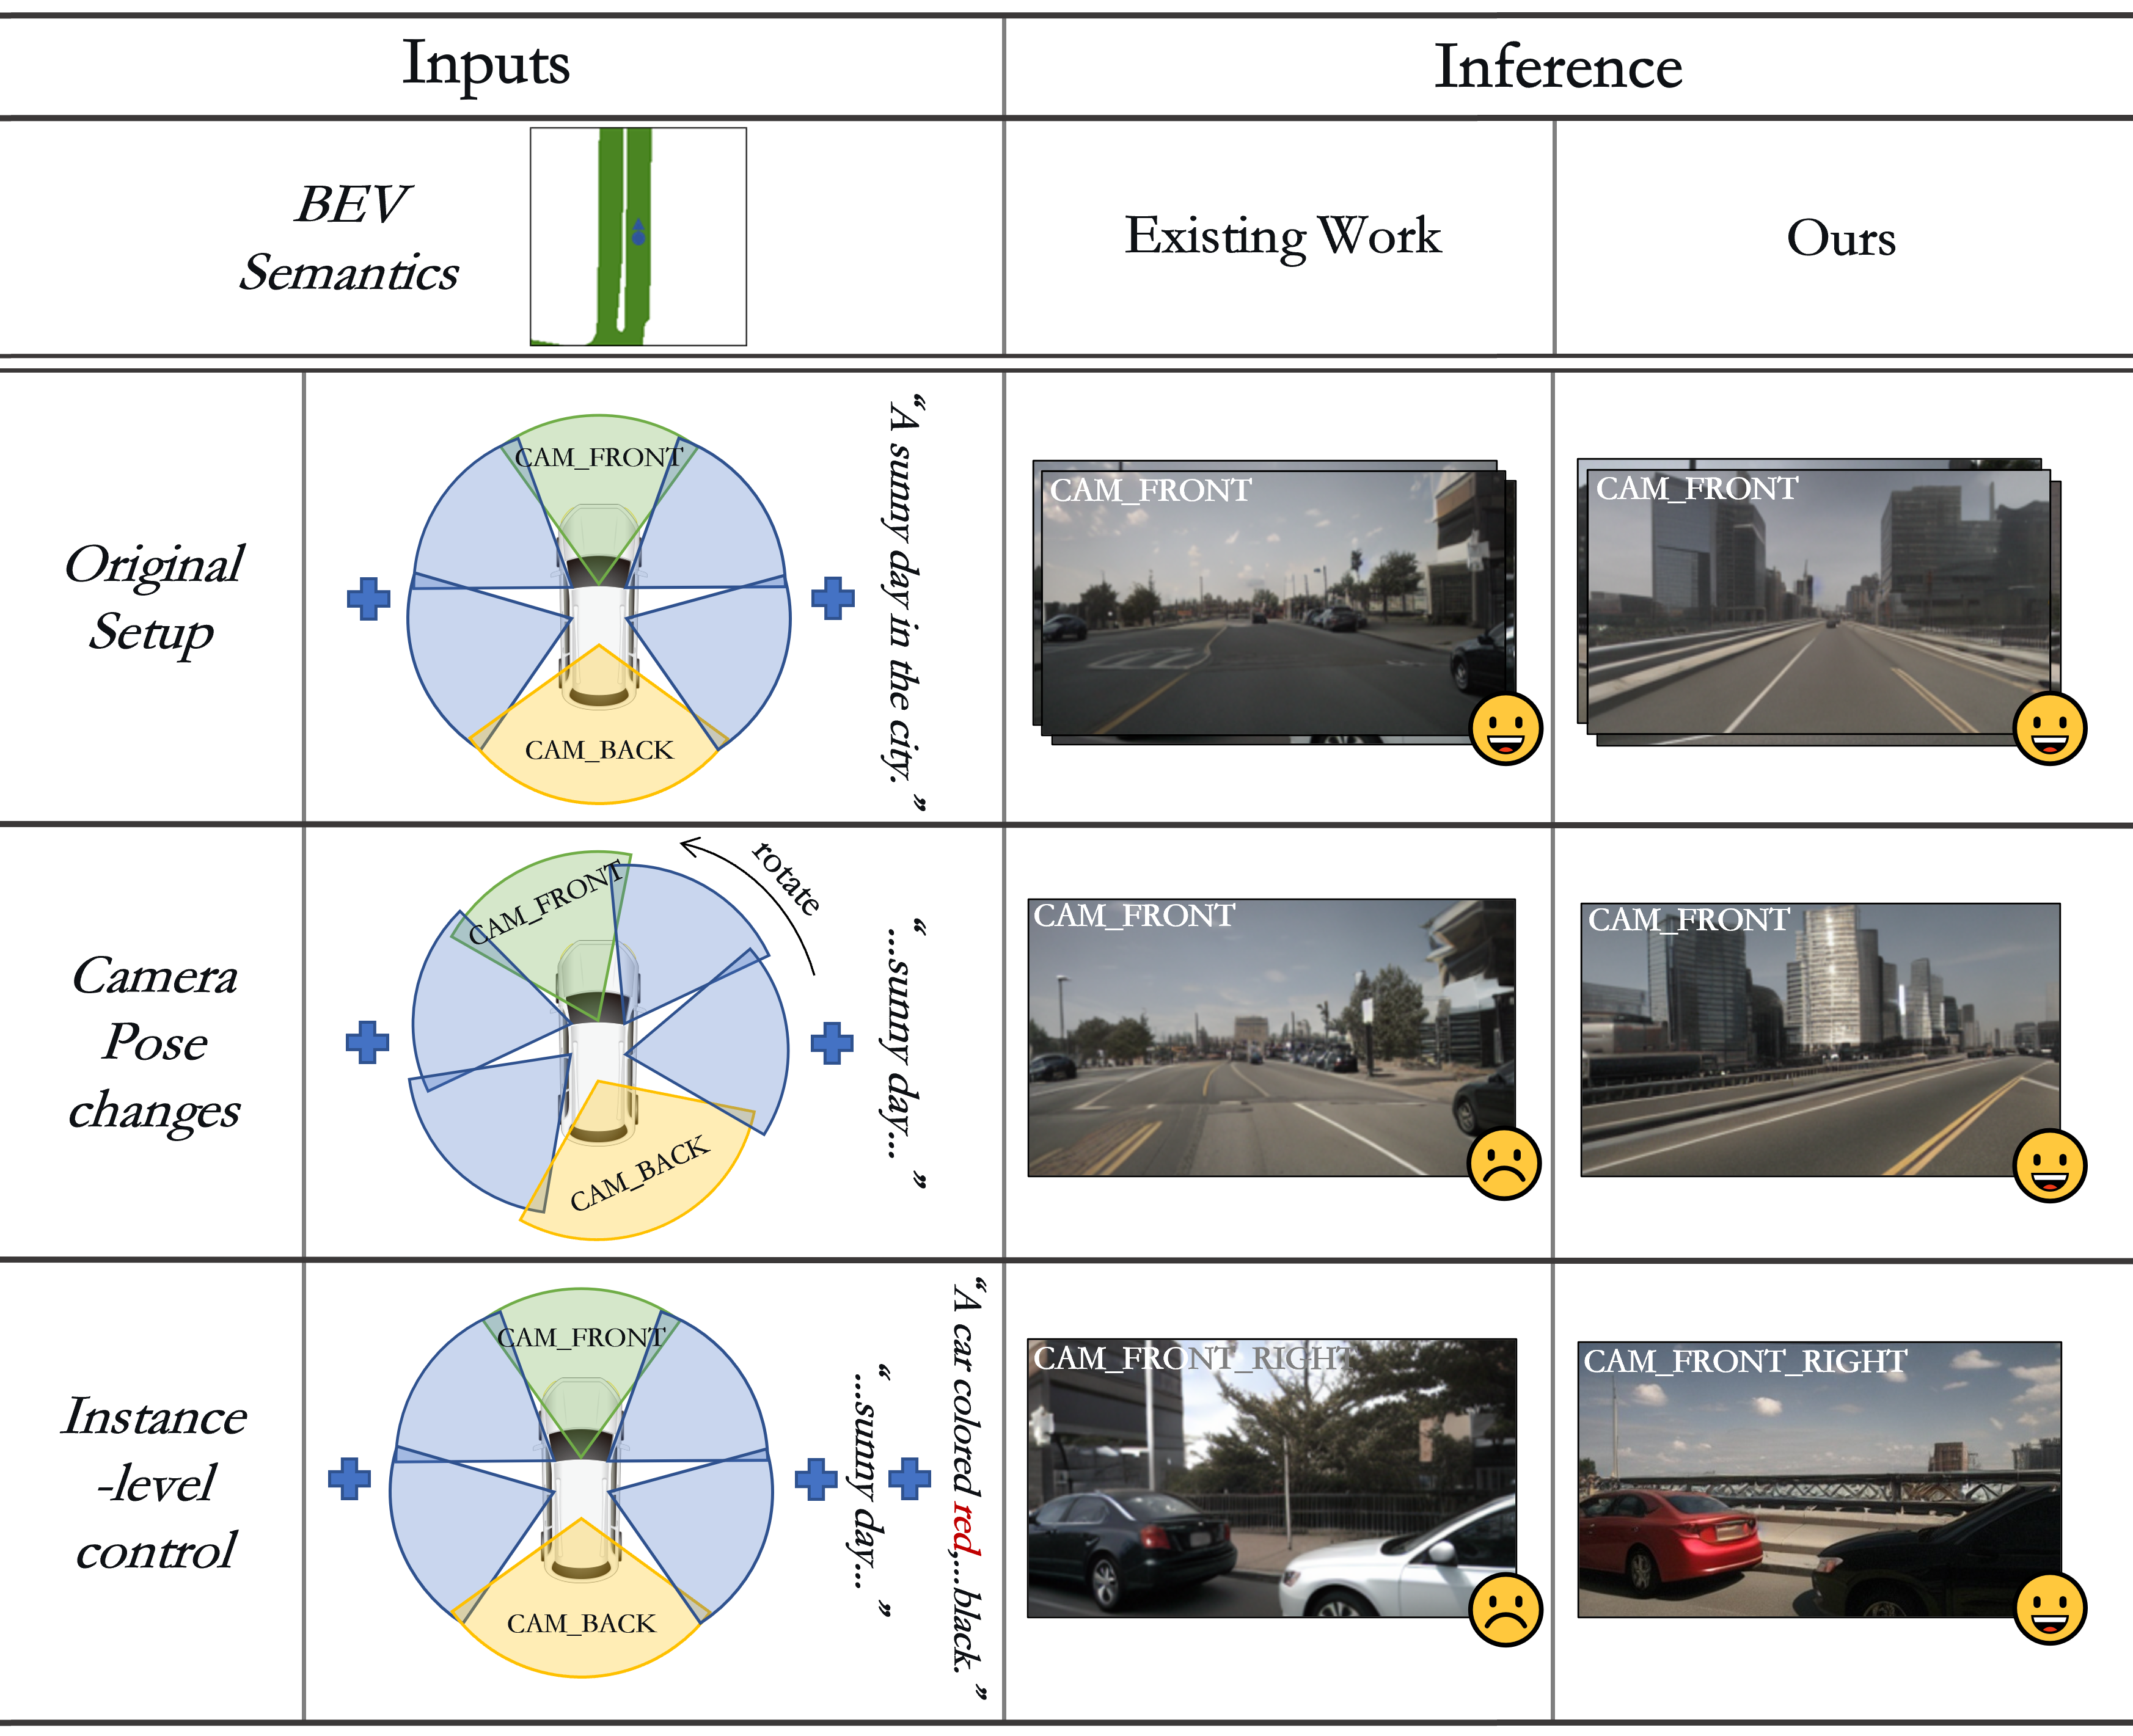
\includegraphics[width=0.9\linewidth]{figures/teaser.png}
\caption{Our MVPbev is able to generate multi-view perspective images with BEV semantics and text prompts. More importantly, MVPbev allows test-time view-point and instance-level control, significantly improving its generalizability. % of existing work.
}
\label{fig:teaser}
\end{figure}
% Thanks to our special initialization and de-nosing processes that explicitly leverage local consistency in latents, MVPbev is able to process perspective semantics in parallel with a pre-trained text-to-image diffusion model and produces multi-view perspective images. Our extensive experiments on NuScenes demonstrate that our method is capable of generating high-resolution photorealistic images from text descriptions with thousands of training samples, surpassing the state-of-the-art methods under various evaluation metrics. We further demonstrate the advances of our method under comprehensive human analysis. Our code and model will be made available.

% or neglect layout consistency, our method MVPbev simultaneously generates images of different perspective views with cross-view awareness, effectively enforcing consistency both visually and semantically. Specifically, our method firstly projects given BEV semantics to perspective view with given camera parameters, which explicitly leverages global semantic coherency. Then we introduce a multi-view attention module to implicitly enforce global consistency among overlapping views w.r.t. cross-view homography. Thanks to our special initialization and de-nosing processes that explicitly leverage local consistency in latents, MVPbev is able to process perspective semantics in parallel with a pre-trained text-to-image diffusion model and produces multi-view perspective images. Our extensive experiments on NuScenes demonstrate that our method is capable of generating high-resolution photorealistic images from text descriptions with thousands of training samples, surpassing the state-of-the-art methods under various evaluation metrics. For instance, our method outperforms ground truth by $4.53$ in terms of PSNR.  We further demonstrate the advances of our method under comprehensive human analysis. Our code and model will be made available.
\end{abstract}



%Then multi-view perspective semantics are stitched together w.r.t. planer assumption to facilitate interactions between various views. Finally, our method processes stitched perspective semantics in parallel with a pre-trained text-to-image diffusion model, while integrating novel homographical loss to enforce global visual consistency. 